\documentclass[10pt,a4paper,twocolumn]{article}

\input{pisika.dat}

%  Editorial staff will uncomment the next line
% \input{staff.hed}


\begin{document}

%--------------------------------------------------------------------------
%  fill in the paper's title, author(s), and corresponding institutions
%--------------------------------------------------------------------------
\providecommand{\ShortAuthorList}[0]{David Beinhauer}
\title{Modelování hledání potravy v mravenčích koloniích}
\author[1,*]{David Beinhauer}
\affil[1]{Přírodovědecká fakulta Univerzity Karlovy, Bioinformatika, Praha, Česká republika}
\affil[*]{david.beinhauer@email.cz}

\date{\dateline{}}

\begin{abstract}
\noindent
%---------------------------------------------------------------------------
%               Include abstract and keywords here
%---------------------------------------------------------------------------
Chování hmyzích druhů žijících v kooperujících koloniích je dodnes 
výzvou pro vědu. Pochopení této problematiky může vést k zdokonalení řešení
řady zdánlivě nesouvisejících problémů. V práci je představen jednoduchý
multiagentní model mravenčí kolonie zaměřující se na problematiku shánění
potravy v různě komplexních prostředích. 
Při analýze byla prokázána schopnost modelu simulace koordinované 
spolupráce mravenců při sbírání potravy.


\DOI{} % do not delete this line
\end{abstract}

\maketitle
\thispagestyle{titlestyle}



%---------------------------------------------------------------------------
%               the main text of your paper begins here
%---------------------------------------------------------------------------
\section{Úvod}

Kolektivní chování řady druhů hmyzu, mezi než patří například mravenci,
je charakteristické komplexností a vysokou koordinovaností jedinců. Kolonie
mravenců například společně zajišťuje potravu pro celou populaci, buduje hnízdo,
strará se o potomky, či se brání před predátory. Pochopení tohoto chování by
mohlo pomoci zdokonalit naše chápání řady biologických systému i nalézt
řešení pro řadu zdánlivě vzdálených problému, mezi něž
patří například problém obchodního 
cestujícího\textsuperscript{\cite{applegate2011traveling}}. 
S ohledem na množství jedinců, komplexnost přirozeného prostředí a 
nepřesnost měřících zařízeních je však exaktní studium chování a 
organizace těchto kolonií velmi komplikované a 
často značně nepřesné. V důsledku nárustu výpočetního výkonu se proto v 
současnosti pro studium takto komplexních dějů stále častěji 
využívají matematické modely\textsuperscript{\cite{drogoul1994multi}, 
\cite{xiang2008ant}, \cite{ilie2013multi}}. 

V této práci navrhujeme a analyzujeme jednoduchý multiagentní model mravenčí 
kolonie zaměřený na problematiku shánění potravy. Model je založen na komunikaci
mravenců pomocí vypouštění a detekce rozdílných hladin feromonu v prostředí.
Z velké části je návrh modelu insporován 
prací\textsuperscript{\cite{jones2010characteristics}}, 
jenž studuje
formování transportních drah plísně 
\emph{Physarum polycephalum}\textsuperscript{\cite{durham1976control}}. 
V analytické části
porovnáváme chování mravenců a jejich úspěšnost při sběru potravy v různě 
strukturovaných prostředích. Dále zkoumáme závislosti počtu jedinců a jejich 
schopnosti dopředu detekovat cílovou destinaci na celkovém množství potravy 
dopraveného do hnízda v průběhu simulace. 


\section{Matematický model}
Při návrhu modelu jsme se zaměřili především na jednoduchou architekturu s
malým množstvím snadno pochopitelných parametrů pro jednodušší analýzu 
fungování modelu.
Ideálně by měl model zachytit kolektivní chování mravenců při hledání potravy.
Mravenci by měli být schopni jednoduchou lokální signalizací pomocí
vypouštění feromonu co nejvíce optimalizovat trasu pro zásobování hnízda
potravou. V modelu je dále možné zkoumat různé varianty map s různě 
rozmístěnými překážkami, hnízdy i potravou. Podrobnější popis modelu
je k nahlédnutí v části \ref{subsec:model_setup}.

\section{Výsledky}

V analýze modelu jsme se zaměřili především na chování mravenců v různých
variantách prostředí. Dále jsme se zaměřili na závislost počtu
jedinců (parametr $n$) a maximální vzdálenosti pro detekci hledaného 
objektu (parametr $d$). Zbylé parametry jsme zvolili pevně na základě
porovnávání výsledků pro různé varianty hodnot (podrobnější popis 
volby parametrů je k nahlédnutí v části \ref{subsec:parameter_choice}).

\subsection{Varianty prostředí}
\label{subsec:map_variants}
Pro analýzu modelu jsme zvolili celkem 6 variant mapy s účelem otestovat
chování modelu v prostředích s odlišnou charakteristikou. Zvolili jsme 
jednotnou velikost mřížky prostředí, jež je rovna $100 \times 100$.
Jednotlivé varianty se liší rozmístěním zdrojů potravy, mraveniště a překážek
v prostředí.

Základní varianta prostředí (ozn. jako \texttt{var-0}), jež je použita 
také pro výběr parametrů, neobsahuje žádnou překážku. Prostředí obsahuje 
jediné mraveniště umístěné přibližně uprostřed mapy a dva zdroje potravy
umístěné v rozích mapy na společné diagonále. Zdroje potravy se od sebe 
mírně liší vzdáleností od hnízda a velikostí. Další varianta 
(ozn. \texttt{var-1}) je téměř identická vůči variantě
\texttt{var-0}. Liší se však v obklopení téměř celého zdroje
potravy překážkami s pouze malým prostorem pro vstup mravenců. Následující
varianta (ozn. \texttt{var-2}) je jednoduché symetrické bludiště s hnízdem 
na levém konci. Okolí hnízda je ohraničeno překážkami, jež vytváří podélný 
průchod pro mravence směrem k potravě. V pravé části mapy je koncipováno 
rozdvojení na jejichž koncích jsou zdroje potravy. Úsek od rozdvojení
k potravě je výrazně kratší než od hnízda k rozdvojení. Velmi podobné je 
rozložení další varianty (\texttt{var-3}). Lišící se od \texttt{var-2} pouze ve 
vzdálenosti hnízda od rozdvojení, která je kratší, a vzdálenostmi rozdvojení od 
zdrojů potravy, které jsou delší. Další z variant (ozn. jako \texttt{var-5})
je v rozložení téměř totožná jako \texttt{var-2}. Liší se pouze v absenci jednoho
ze zdrojů potravy. Poslední varianta (ozn. jako
\texttt{var-4}) je koncipována jako průchod ve středu mapy s konci 
obsahujícími zdroje potravy. Hnízdo je umístěno ve středu mapy a je 
podélně ohraničeno překážkami vytvářející průchod. Na levém a pravém konci
mapy jsou umístěny zdroje potravy. Obrázek \ref{fig:map_variants}
nabízí grafické znázornění rozložení variant prostředí.
 

\begin{figure}[tb]
  \centering
  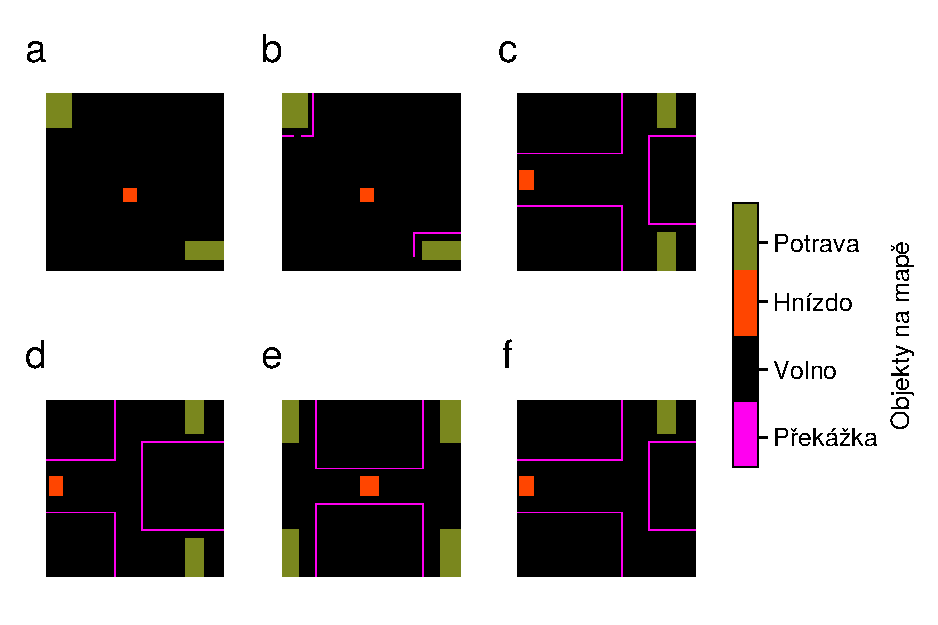
\includegraphics[width=0.98\linewidth]{images/maze_variants.pdf}
  \caption{\textbf{Varianty prostředí modelu:} 
  Zobrazení variant prostředí modelu použitých v experimentech. 
  Barevně rozlišujeme objekty v prostředí (viz. legenda).
  \textbf{a} Varianta \texttt{var-0}, 
  \textbf{b} varianta \texttt{var-1},
  \textbf{c} varianta \texttt{var-2},
  \textbf{d} varianta \texttt{var-3},
  \textbf{e} varianta \texttt{var-4},
  \textbf{f} varianta \texttt{var-5}.}
  \label{fig:map_variants}
\end{figure} 



\subsection{Porovnání variant prostředí}
\label{subsec:variant_comparision}

V rámci kontroly správného fungování modelu a pochopení strategie chování 
mravenců jsme nejprve spustili 4000 iterací simulace modelu na všech 
variantách prostředí pro 400 mravenců (parametr $n$) a pro maximální
vzdálenost detekce 10 (parametr $d$). Hodnoty parametrů $n$ a $d$ 
jsme volili tak, aby problém sbírání
potravy nebyl příliš jednoduchý a nezajišťoval vždy téměř stoprocentní
sesbírání potravy (vysoké hodnoty parametrů $n$ a $d$). Zároveň však
požadujeme, aby chování mravenců nebylo příliš náhodné 
(příliš nízké hodnoty parametrů $n$ a $d$). Na základě opakovaného 
běhu simulací modelu a animací chování simulacce pro různé hodnoty 
parametrů $n$ a $d$ jsme se rozhodli pro volbu parametrů popsanou výše. 
Zbylé parametry jsme nastavili na hodnoty, jež jsou popsány v části 
\ref{subsec:experiment_describtion}. 

S takto zvolenými parametry jsme následně pozorovali chování modelu na základě 
rozložení hladin variant feromonů a animacích pohybu mravenců v různých 
variantách prostředí. Na obrázcích \ref{fig:pheromones_300}, 
\ref{fig:pheromones_1000} a \ref{fig:pheromones_4000} 
mužeme nahlédnout na rozložení hladin feromonů na 
různých pozicích v daných prostředích po $300$, $1000$ a $4000$ 
iteracích simulace modelu. Pro lepší pochopení je vhodné porovnat 
tyto obrázky s návrhy jednotlivých prostředí znázorněných na obrázku
\ref{fig:map_variants}.

Téměř u všech variant prostředí pozorujeme vyšší koncentraci feromonu typu
\texttt{food} v okolí hnízda a feromonu typu \texttt{nest} v 
okolí zdrojů potravy. Tato vlastnost je pravděpodobně dána 
vyšší koncentrací mravenců mířících k potravě v okolí hnízda 
(všichni mravenci vyrážejí hledat potravu ze stejného mraveniště) a 
naopak vyšší koncentrací vracejících se mravenců v okolí zdroje
potravy (z analogického důvodu jako v případě vyrážejících mravenců).

Varianty \texttt{var-0} a \texttt{var-1} se liší pouze v rozestavení 
překážek okolo zdrojů potravy. Proto je rozložení hladin feromonů mezi
těmito variantami především v počáteční fázi simulace velmi podobné
(viz. obrázek \hyperref[fig:pheromones_300]{\ref*{fig:pheromones_300}a, b}). 
Po uplynutí více iterací 
simulace však můžeme nahlédnout, že v případě varianty \texttt{var-1}
je hladina feromonu typu \texttt{food} 
rovnoměrněji rozprostřena v prostředí než u
varianty \texttt{var-0}, v níž jsou feromony koncentrovány více kolem optimálních
cest mezi zdroji potravy a hnízdem (viz. obrázky 
\hyperref[fig:pheromones_1000]{\ref*{fig:pheromones_1000}a, b}
a \hyperref[fig:pheromones_4000]{\ref*{fig:pheromones_4000}a, b}). 
Tuto skutečnost
si odůvodňujeme vyšší mírou náhodného prohledávání prostředí mravenci
v případě varianty \texttt{var-1}, jelikož nalezení cesty k potravě
je náročnější z důvodu umístění překážky téměř okolo celého obvodu
zdrojů potravy. Tato hypotéza je podpořena také animacemi simulací 
(viz. doplňové materiály S1, S2).

Podobně jako v předchozím přídadě stojí za zmínku porovnat chování
podobných variant \texttt{var-2}, \texttt{var-3} a \texttt{var-5}. 
V případě 300 a 1000 iterací jsou tyto varianty od sebe téměř 
nerozlišitelné (viz. obrázky \hyperref[fig:pheromones_300]{\ref*{fig:pheromones_300}c, d, f}
a \hyperref[fig:pheromones_1000]{\ref*{fig:pheromones_1000}c, d, f}). Po 4000
iteracích se však rozdíly v hladinách feromonů již výrazně 
odlišují (viz. \hyperref[fig:pheromones_4000]{\ref*{fig:pheromones_4000}c, d, f}).

Při porovnání variant \texttt{var-2} a \texttt{var-5}, jež se liší
pouze slepým ramenem ve variantě \texttt{var-5}, můžeme sledovat, že
ve variantě \texttt{var-5} je pozorovatelně vyšší hladina feromonu
typu \texttt{nest} v rameni se zdrojem potravy oproti oběma ramenům
ve variantě \texttt{var-2}. Tato skutečnost vypovídá
o vyšší koncentraci mravenců v rameni s potravou v porovnání s oběma
rameny s potravou v případě \texttt{var-2} a je tedy i částečným 
potvrzením správného chování mravenců (očekáváme, že se budou 
spíše koncentrovat v okolí potravy než ve slepém rameni). Podobný jev
lze pozorovat i v případě \texttt{var-3}, lišící se od \texttt{var-2}
pouze v poměru jednotlivých délek ramen bludiště (křižovatka je blíže 
hnízdu a zdroje potravy dále od křižovatky). I v tomto případě jsou
koncentrace feromonů přibližně stejné v obou větvích (mírný rozdíl 
v koncentracích přisuzujeme náhodnému výběru mezi větvemi, 
jenž je způsoben návrhem modelu). 

Zajímavé je porovnání hladin feromonu typu \texttt{nest} mezi variantami 
\texttt{var-2} a \texttt{var-3} v ramenech se zdrojem potravy. 
V případě \texttt{var-2} je tato hladina výrazně nižší než v případě
\texttt{var-3}. Tento jev je pravděpodobně způsoben rozdílnou délkou 
ramen. V případě kratších ramen se zdrojem potravy 
(\texttt{var-2}) mravenci velmi rychle zamíří ke křižovatce ramen,
kde je typicky vyšší koncetrace feromonu, protože se zde slévají
hladiny feromonu mravenců navrácejících se z obou ramen. Naopak v 
případě delších ramen s potravou (\texttt{var-3}). Nejsou mravenci
tak silně přitahování ke křižovatce a mohou tvořit cyklické skupinky
navzájem se ovlivňujících vracejících se mravenců v jednotlivých 
ramenech. 

Problém vzniku cyklických skupinek navzájem se ovlivňujících
mravenců lze také pozorovat u variant \texttt{var-2}, \texttt{var-3} i 
\texttt{var-5} v místě křižovatky ramen, kde je typicky
vysoká koncetrace jak feromonu typu \texttt{nest}, tak i typu 
\texttt{food}, což svědčí o velké koncentraci mravenců navrácejících
se do hnízda i hledajících potravu. Popsané vlastnosti chování mravenců
ve variantách \texttt{var-2}, \texttt{var-3} a \texttt{var-5} jsou
podpořeny také i animacemi simulací (viz. doplňové materiály S3, S4, S6).

Poslední varianta \texttt{var-4} prokazuje podobné vlastnosti 
jaké jsme již popisovali v předchozích variantách 
\texttt{var-2}, \texttt{var-3} a \texttt{var-5}. Můžeme zde však ještě 
výrazněji nahlédnout na tvoření cyklických skupinek navrácejících
se mravenců, jež je způsobeno větším množstvím zdrojů potravy, menšími skupinkami
mravenců v jednotlivých větvích a tedy také větším vlivem mezi 
jednotlivými mravenci (viz. obrázky 
\hyperref[fig:pheromones_300]{\ref*{fig:pheromones_300}e}, 
\hyperref[fig:pheromones_1000]{\ref*{fig:pheromones_1000}e} a 
\hyperref[fig:pheromones_4000]{\ref*{fig:pheromones_4000}e}
a doplňové materiály S5).


\begin{figure}[tb]
  \centering
  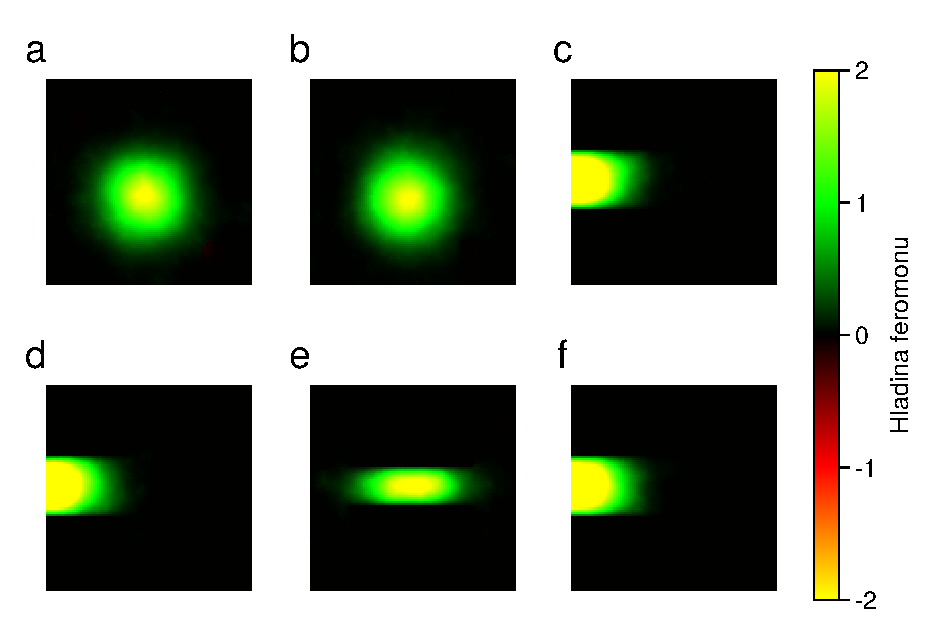
\includegraphics[width=0.98\linewidth]{images/pheromone_levels_300.pdf}
  \caption{\textbf{Hladina feromonu po 300 iteracích simulace modelu:} 
  Kombinace hladin feromonů obou typů v různých variantách prostředí 
  po 300 iteracích algoritmu. 
  Absolutní hodnota hladiny feromonu značí součet hladin obou variant
  feromonů. Znaménko hladiny feromonu je dáno
  feromonem s vyšší koncentrací (záporné (červené odstíny) - vyšší 
  koncentrace feromonu typu \texttt{nest} (navrácející se mravenci), 
  kladné - více feromonu typu \texttt{food} (hledající potravu)). 
  Oblasti se žlutým odstínem jsou oblasti s vysokou 
  koncentrací obou typů feromonů.
  \textbf{a} Varianta \texttt{var-0}, 
  \textbf{b} varianta \texttt{var-1},
  \textbf{c} varianta \texttt{var-2},
  \textbf{d} varianta \texttt{var-3},
  \textbf{e} varianta \texttt{var-4},
  \textbf{f} varianta \texttt{var-5}.}
  \label{fig:pheromones_300}
\end{figure}

\begin{figure}[tb]
  \centering
  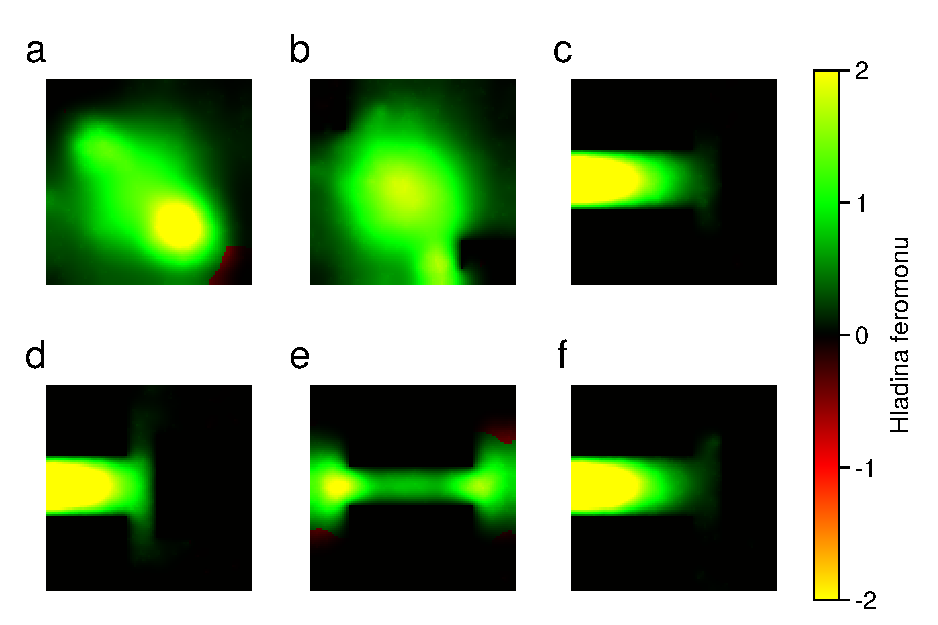
\includegraphics[width=0.98\linewidth]{images/pheromone_levels_1000.pdf}
  \caption{\textbf{Hladina feromonu po 1000 iteracích simulace modelu:} 
  Kombinace hladin feromonů obou typů v různých variantách prostředí 
  po 1000 iteracích algoritmu. Význam hladiny feromonu je podrobněji
  popsán v popisku obrázku \ref{fig:pheromones_300}.
  \textbf{a} Varianta \texttt{var-0}, 
  \textbf{b} varianta \texttt{var-1},
  \textbf{c} varianta \texttt{var-2},
  \textbf{d} varianta \texttt{var-3},
  \textbf{e} varianta \texttt{var-4},
  \textbf{f} varianta \texttt{var-5}.}
  \label{fig:pheromones_1000}
\end{figure}

\begin{figure}[tb]
  \centering
  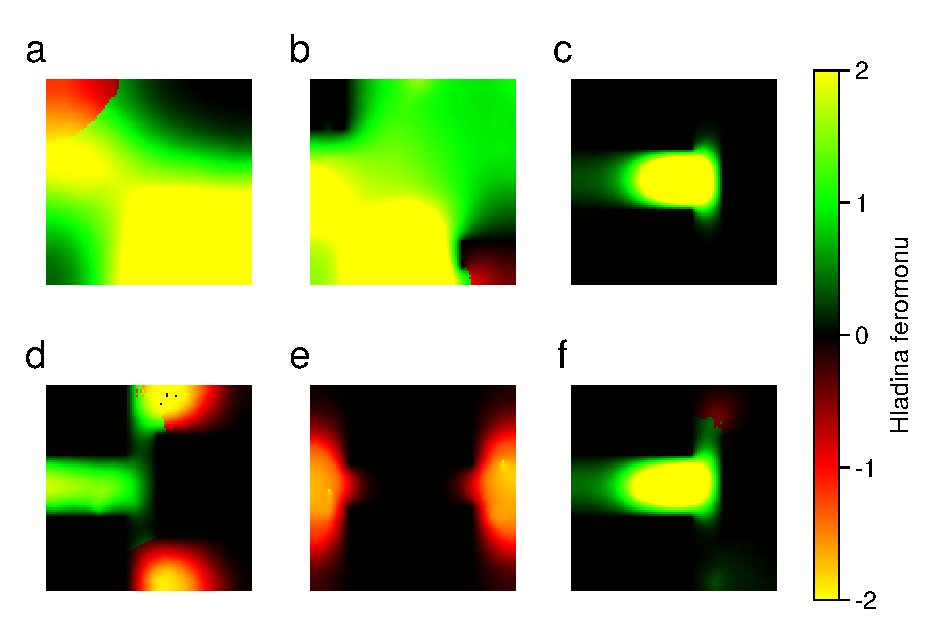
\includegraphics[width=0.98\linewidth]{images/pheromone_levels_4000.pdf}
  \caption{\textbf{Hladina feromonu po 4000 iteracích simulace modelu:} 
  Kombinace hladin feromonů obou typů v různých variantách prostředí 
  po 4000 iteracích algoritmu. Význam hladiny feromonu je podrobněji
  popsán v popisku obrázku \ref{fig:pheromones_300}.
  \textbf{a} Varianta \texttt{var-0}, 
  \textbf{b} varianta \texttt{var-1},
  \textbf{c} varianta \texttt{var-2},
  \textbf{d} varianta \texttt{var-3},
  \textbf{e} varianta \texttt{var-4},
  \textbf{f} varianta \texttt{var-5}.}
  \label{fig:pheromones_4000}
\end{figure}



\subsection{Různý počet mravenců}

Jedním ze zkoumaných parametrů byl počet mravenců v modelu (parameter
$n$), který jsme zkoumali při nastavení parametrů modelu popsaném v části 
\ref{subsec:experiment_describtion} a pro parametr maximální
hloubky detekce s hodnotou $d=10$.

Nahlédli jsme, že volba parametru $n$ výrazně neovlivňuje 
množství sesbírané potravy v různých variantách prostředí 
(viz. obrázek \ref{fig:num_ants_means}). Můžeme také usuzovat, že v případě 
proměnlivého parametru $n$ jsou nejobtížnější varianty pro
sesbírání potravy varianty \texttt{var-2}, \texttt{var-3} a \texttt{var-5}.
Naopak v případě variant \texttt{var-0}, \texttt{var-1} a \texttt{var-4}
jsou v průměru sesbírány téměř veškeré zásoby potravy v prostředí.
Překvapivé jsou především výsledky pro \texttt{var-4}, které prokazují
dokonce lepší výsledky něž v případě \texttt{var-1}. Tento fakt je 
částečně v rozporu s poznatky z části \ref{subsec:variant_comparision},
které odhadovaly zacyklení mravenců v okolí křižovatek a pravděpodobně
také snížení celkového množství sesbírané potravy (část mravenců
by vlivem zacyklení nikdy nedorazila do cíle). Důvodem rozdílných 
výsledků je pravděpodobně vyšší počet mravenců v průměrném případě 
oproti zkoumanému počtu $n=400$ ve zmíněné části.

Poznatky zmíněné výše jsou také podpořeny závislostí sesbírané potravy 
na počtu mravenců při různých variantách (viz. obrázky 
\ref{fig:num_ants_together} a \ref{fig:num_ants_separated}).
Na základě těchto závislostí můžeme nahlédnout, že při hodnotě 
parametru $n$ okolo hodnoty $500$ a výše, již téměř nedochází k nárustu
sesbírané potravy. Typicky buď dochází k sesbírání veškeré potravy, 
nebo k ustálení na určité části celkového počtu a zbylou část
potravy téměř není možné sesbírat ani s vyšší počtem mravenců. 
K tomuto jevu dochází především při již zmíněných variantách 
\texttt{var-2}, \texttt{var-3} a \texttt{var-5}, zde pravděpodobně
dochází k zacyklení části navrácejících se mravenců na křižovatkách
ramen a tím pádem k nemožnosti dopravit potravu do hnízda. Nejhůře v 
tomto ohledu dopadla varianta \texttt{var-3} s delšími rameny 
ke zdrojům potravy, kde pravděpodobně dochází k zacyklení mravenců ještě 
v jednotlivých ramenech. Nedosáhnou tak často ani křižovatky, kde je 
vyšší šance odtržení od cyklické skupinky a návratu do hnízda, jelikož
je hnízdo v křižovatce blíže a není schováno za překážkou. Je tak možné,
že bude v dostatečné blízkosti pro detekci mravencem a jeho odtržení od
vlivu dalších mravenců. Dalším ze zajímavých poznatků je vyšší závislost
na parametru $n$ ve variantě \texttt{var-1}, způsobena pravděpodobně
malým prostorem pro průchod mravenců k překážce.

\begin{figure}[tb]
  \centering
  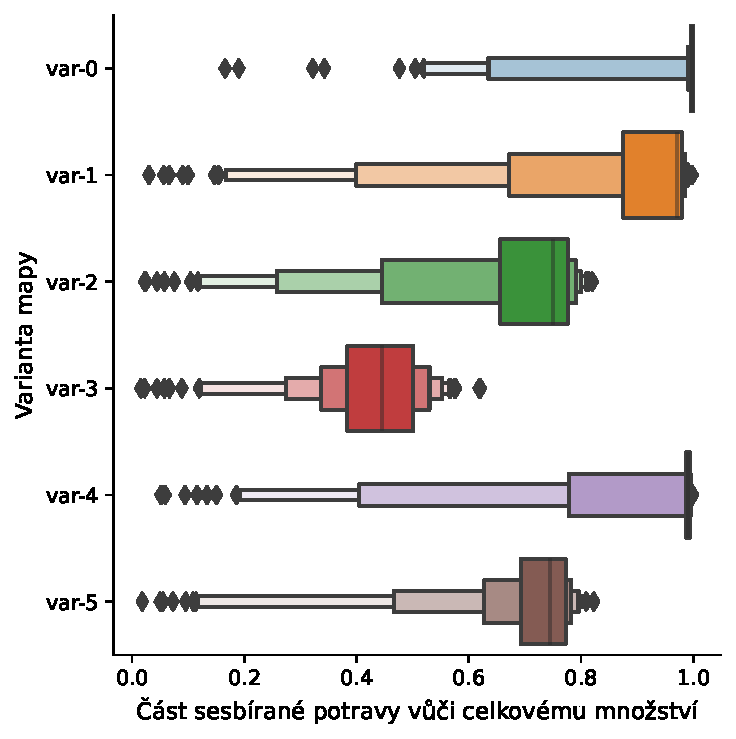
\includegraphics[width=0.98\linewidth]{images/num_ants_variants_means.pdf}
  \caption{\textbf{Porovnání množství sesbírané potravy mezi variantami mapy s promněnlivým počtem mravenců:}
  Znázornění distribuce množství sesbírané potravy mravenci 
  při různém počtu mravenců (parametr $n$).}
  \label{fig:num_ants_means}
\end{figure}

\begin{figure}[tb]
  \centering
  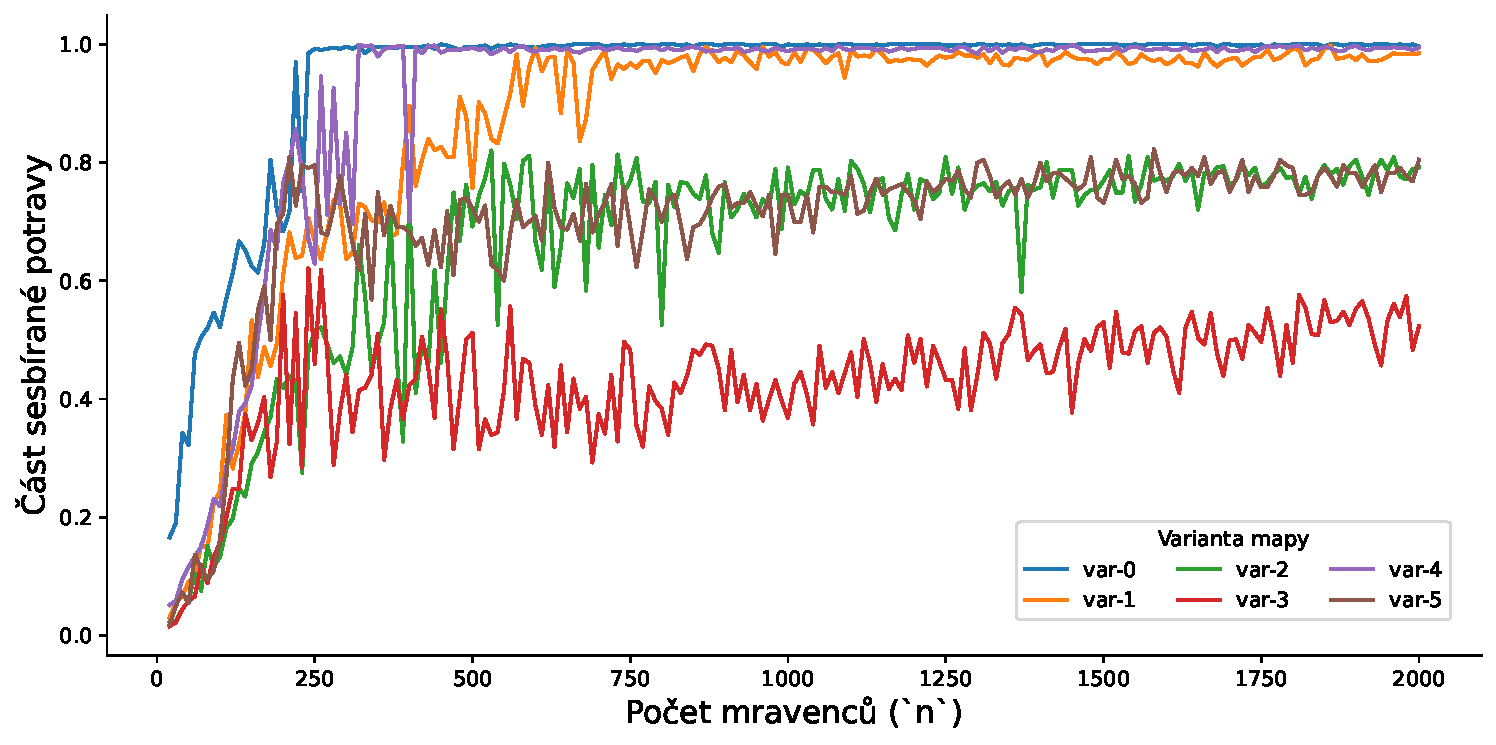
\includegraphics[width=0.98\linewidth]{images/num_ants_variants_together.pdf}
  \caption{\textbf{Množství sesbírané potravy v závislosti na počtu mravenců:}
  Porovnání závislostí množství sesbírané potravy na počtu 
  mravenců $n$ mezi variantami prostředí.}
  \label{fig:num_ants_together}
\end{figure}

\begin{figure}[tb]
  \centering
  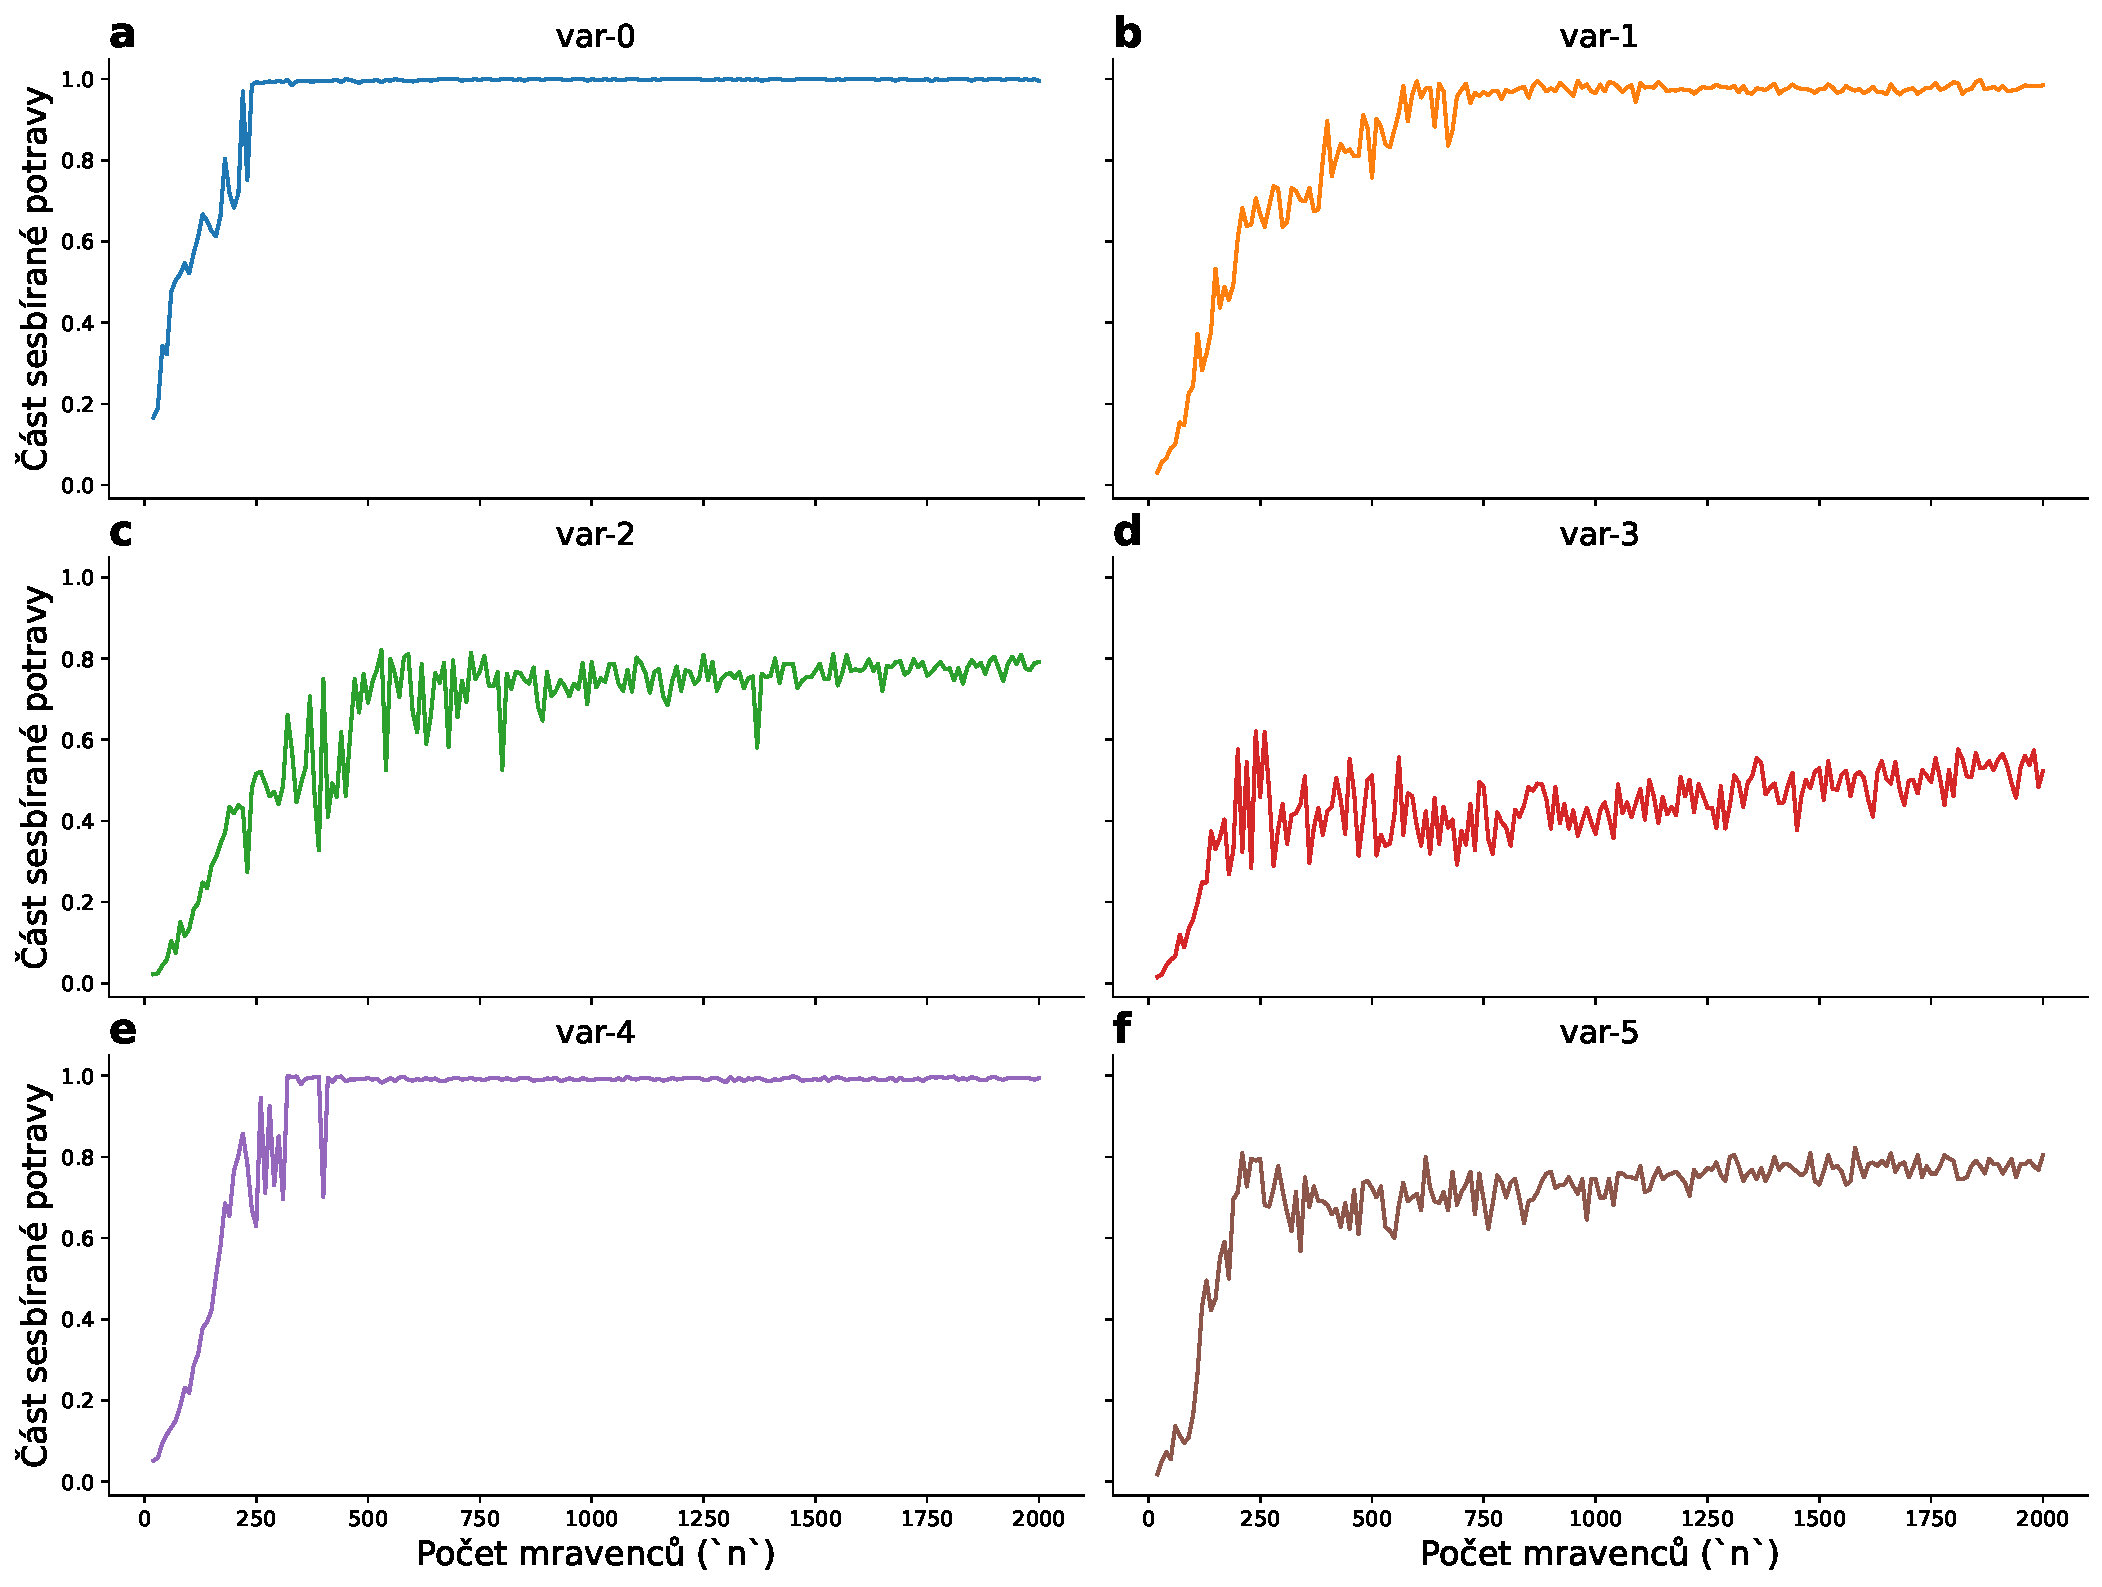
\includegraphics[width=0.98\linewidth]{images/num_ants_variants_separated.pdf}
  \caption{\textbf{Množství sesbírané potravy v závislosti na počtu mravenců:}
  Závislosti množství sesbírané potravy na počtu 
  mravenců $n$ při různých variantách prostředí. \textbf{a}-\textbf{f} 
  Znázornění výsledků pro jednotlivé varianty prostředí, jejichž název je popsán
  v příslušném grafu.}
  \label{fig:num_ants_separated}
\end{figure}



\subsection{Různá vzdálenost detekce objektu}

Posledním zkoumaným parametrem je závislost maximální vzdálenosti
pro detekci cílového objektu (potrava, hnízdo) (parametr $d$).
Nastavení parametrů je podrobněji popsáno v části 
\ref{subsec:experiment_describtion}. Počet mravenců jsme zvolili 
$n=400$.

Na rozdíl od parametru $n$ je množství sesbírané potravy především
ve variantách \texttt{var-4} a \texttt{var-5} výrazně závislé na
volbě parametru $d$ (viz. obrázek \ref{fig:search_depth_means}).
Na základě průměrného množství sesbírané potravy dopadla nejhůře
varianta \texttt{var-2} následována \texttt{var-3} a \texttt{var-5}.

Závislost parametru $d$ na množství sesbírané potravy můžeme 
sledovat u všech variant prostředí (viz. obrázky 
\ref{fig:search_depth_together} a \ref{fig:search_depth_separated}).
Zvláštní chování můžeme sledovat v případě varianty \texttt{var-5},
v níž množství sesbírané potravy výrazně osciluje v závislosti
na $d$ (viz. obrázek \ref{fig:search_depth_separated}) a oproti 
podobným variantám \texttt{var-2} a \texttt{var-3} se značně 
odlišuje a v průměru jsou výsledky při této variantě lepší. 
Tuto skutečnost si odůvodňujeme slepým ramenem, tedy také
vyšší koncetrací mravenců mířících stejným směrem a tedy vyšší šancí 
následování správné cesty (nerozdělí se k různým zdrojům potravy).



\begin{figure}[tb]
  \centering
  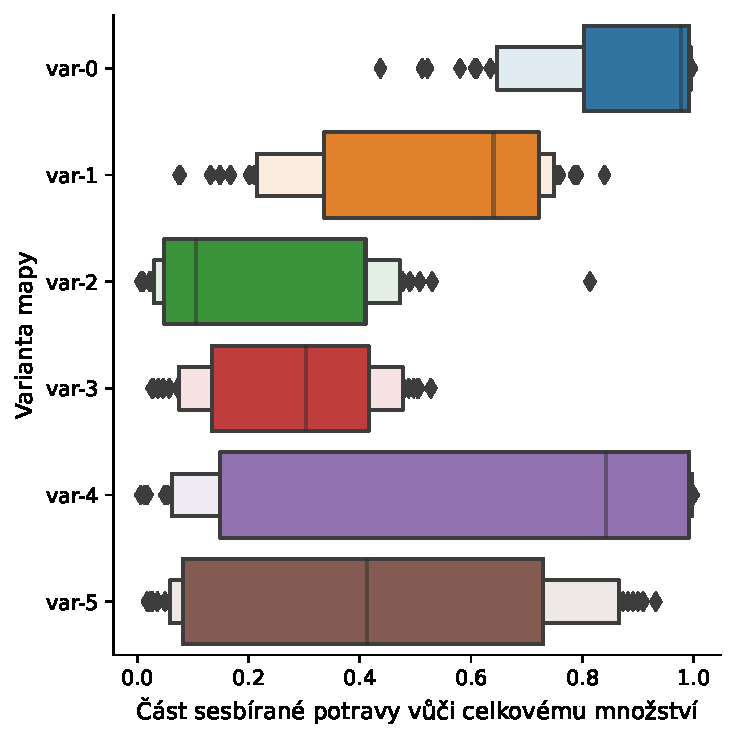
\includegraphics[width=0.98\linewidth]{images/search_depth_variants_means.pdf}
  \caption{\textbf{Porovnání množství sesbírané potravy mezi variantami mapy s promněnlivou hloubkou prohledávání:}
  Znázornění distribuce množství sesbírané potravy mravenci 
  při různé maximální vzdálenosti detekce cílového objektu (parametr $d$).}
  \label{fig:search_depth_means}
\end{figure}

\begin{figure}[tb]
  \centering
  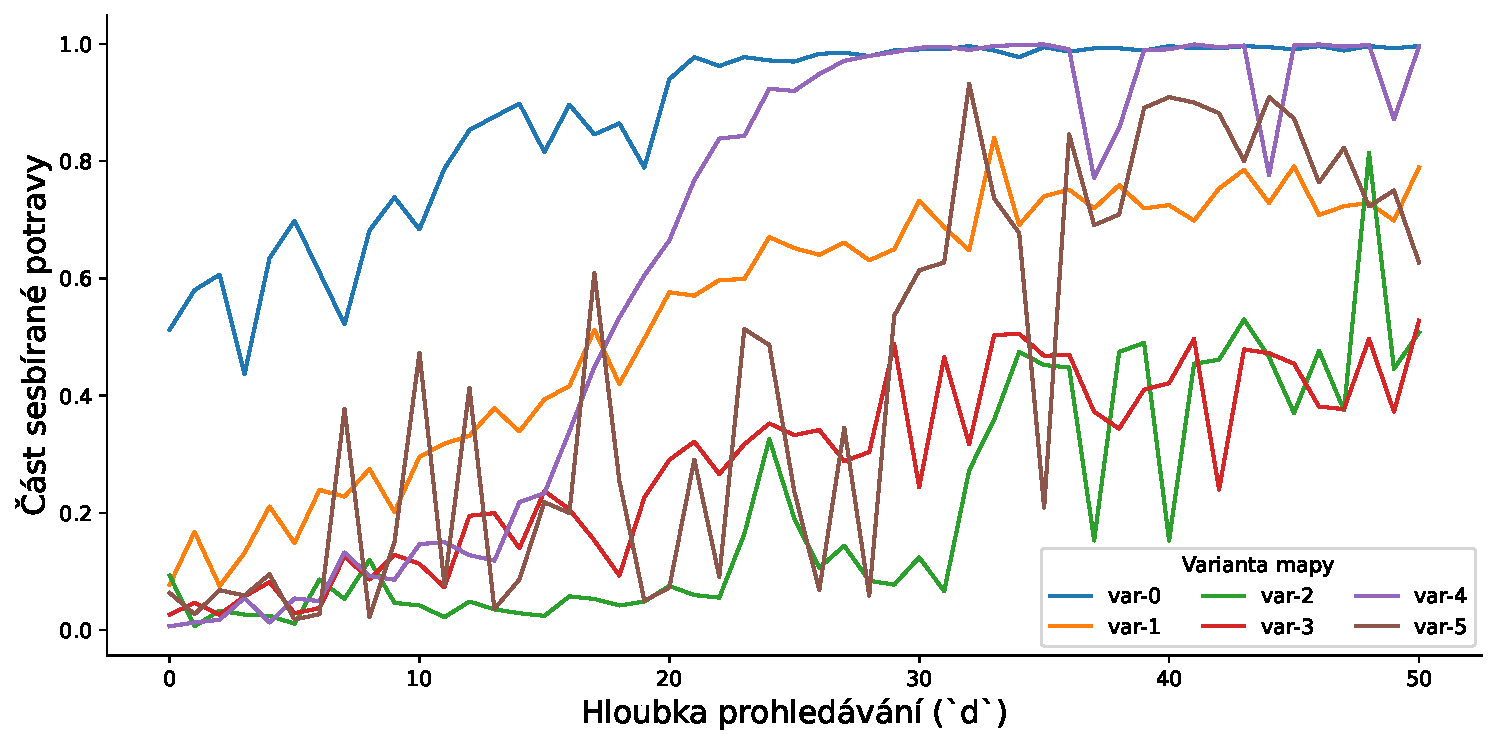
\includegraphics[width=0.98\linewidth]{images/search_depth_variants_together.pdf}
  \caption{\textbf{Množství sesbírané potravy v závislosti na hloubce prohledávání:}
  Porovnání závislostí množství sesbírané potravy 
  při různé maximální vzdálenosti detekce cílového objektu (parametr $d$).}
  \label{fig:search_depth_together}
\end{figure}

\begin{figure}[tb]
  \centering
  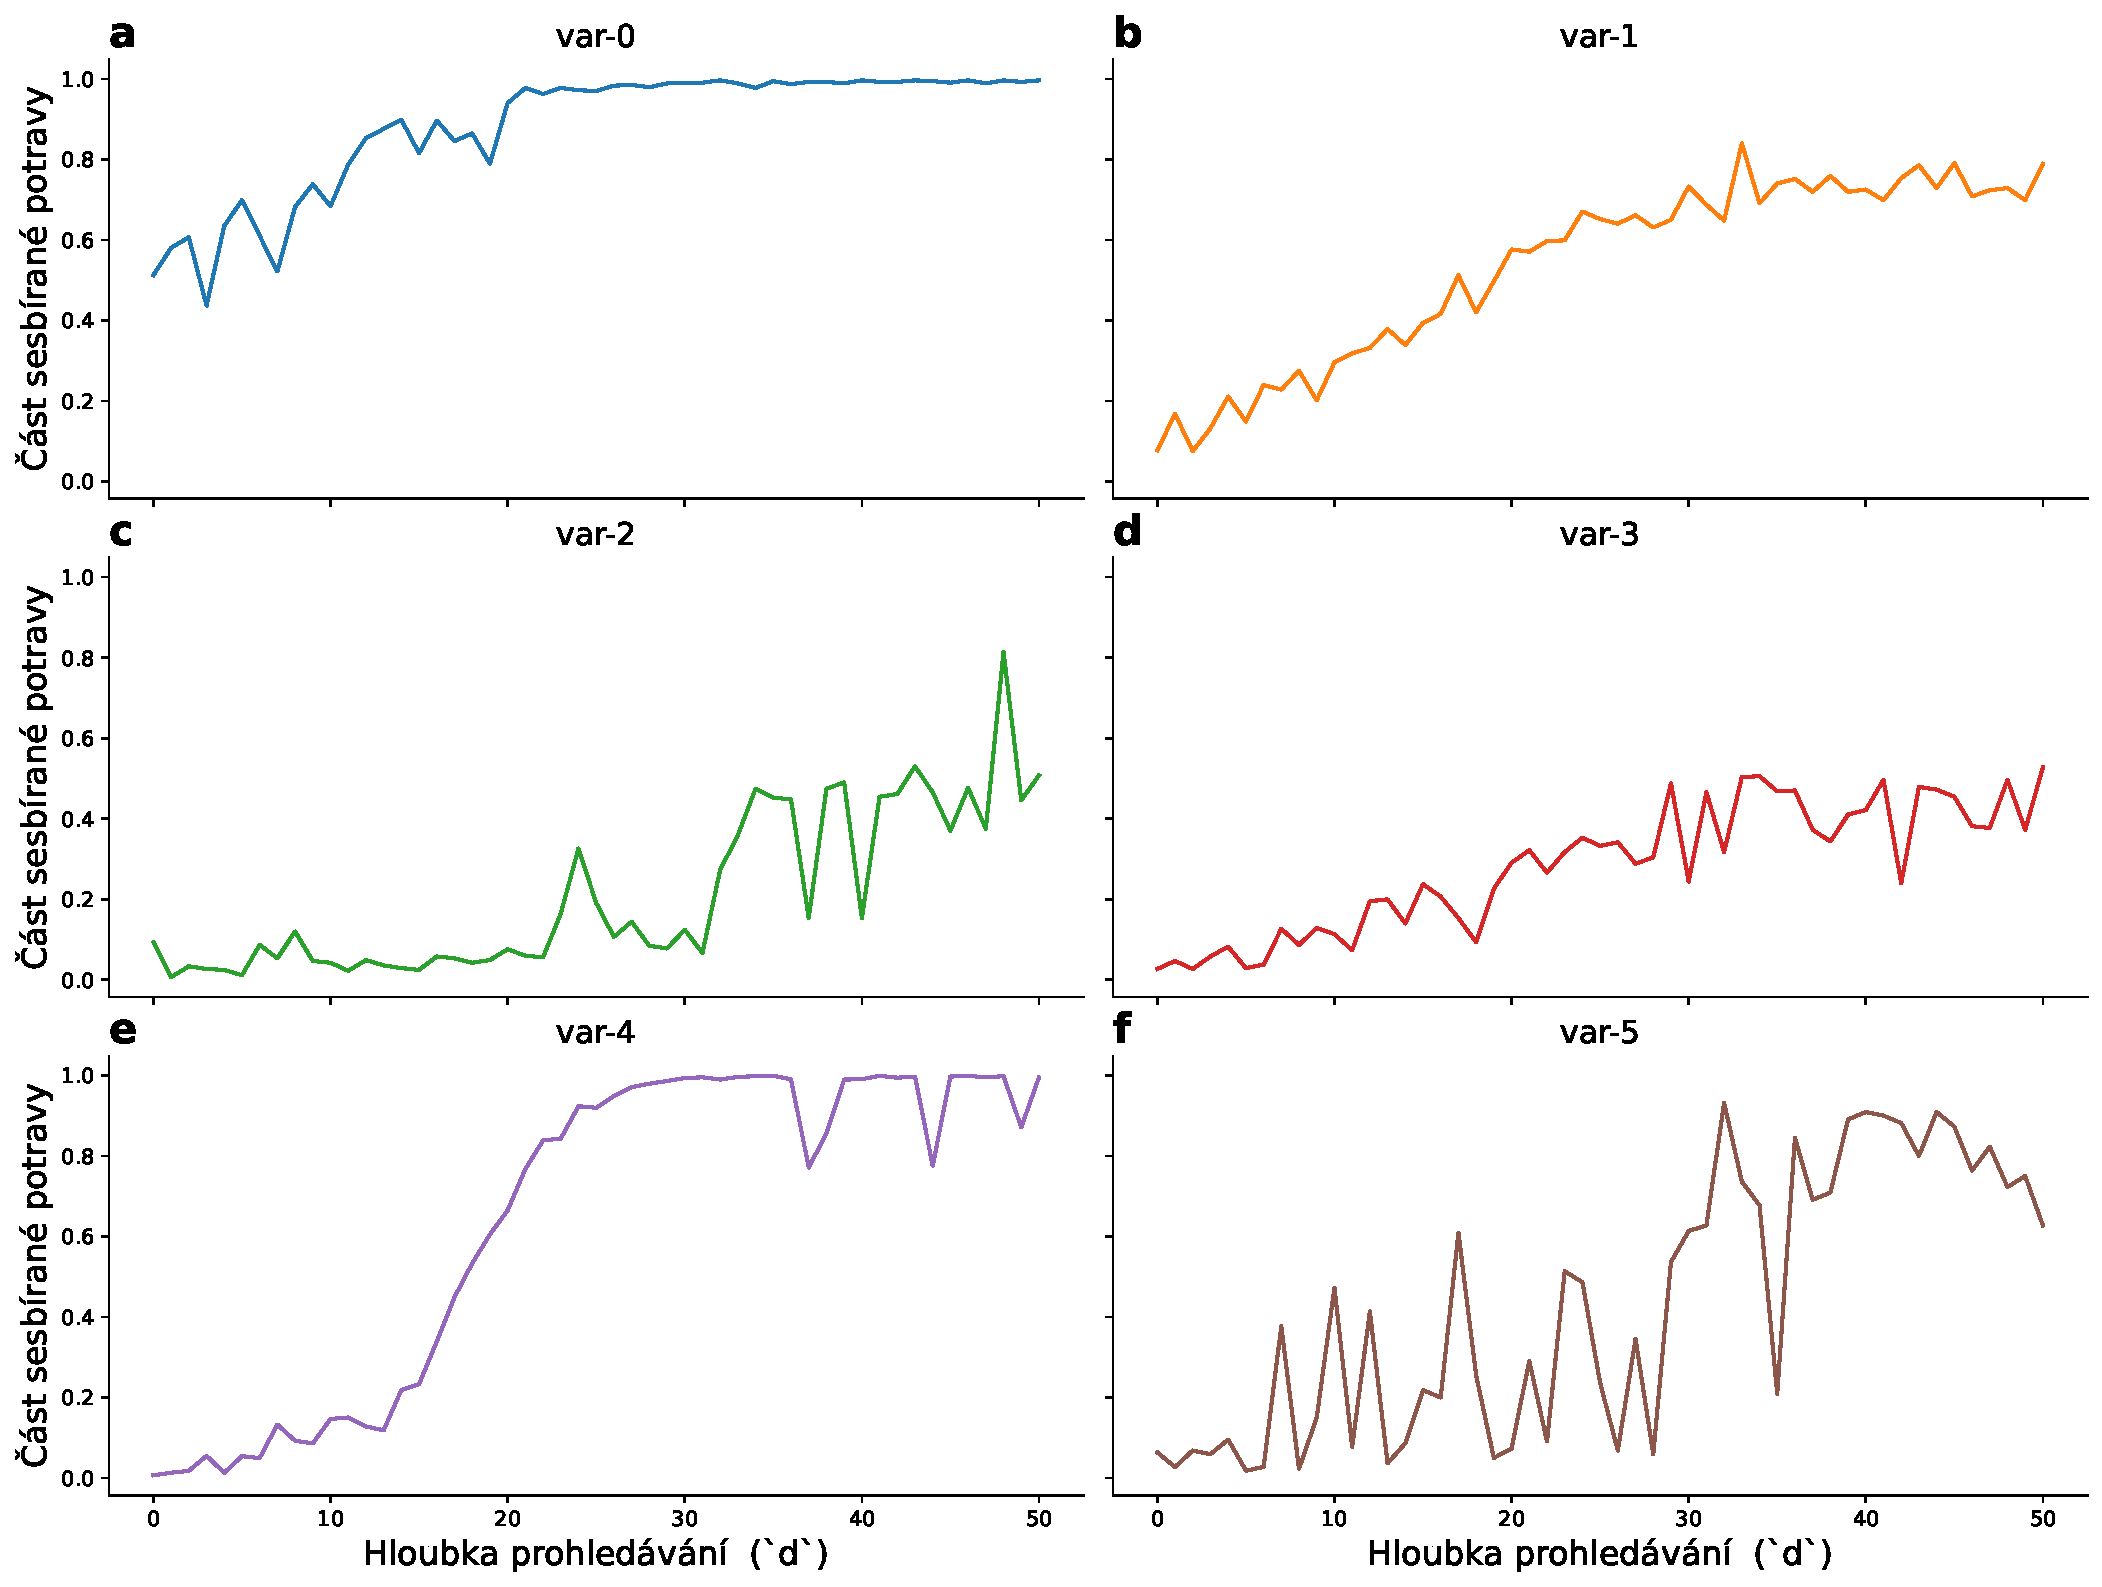
\includegraphics[width=0.98\linewidth]{images/search_depth_variants_separated.pdf}
  \caption{\textbf{Množství sesbírané potravy v závislosti na hloubce prohledávání:}
  Závislosti množství sesbírané potravy
  při různé maximální vzdálenosti detekce cílového objektu (parametr $d$).
  \textbf{a}-\textbf{f} 
  Znázornění výsledků pro jednotlivé varianty prostředí, jejichž název je popsán
  v příslušném grafu.}
  \label{fig:search_depth_separated}
\end{figure}


\section{Diskuze}
Navržený model dokázal ve většině případů vhodně simulovat kolektivní
chování mravenců s rozumnou úspěšností sesbírání potravy. Během analýzy 
jsme narazili na významnou závislost volby zkoumaného prostředí a 
nastavení parametru maximální vzdálenosti detekce hledaného objektu
(parametr $d$). Podrobnější zaměření na tyto parametry by mohlo být 
předmětem zkoumání navazujících prací. 

Dále jsme vypozorovali častý vznik navzájem se ovlivňujících skupinek 
mravenců vedoucí k zacyklení pohybu mravenců, jež vedlo k významnému
poklesu kvality chování mravenců. Eliminace vzniku tohoto
fenoménu v modelu by mohlo vézt k výraznému nárustu kvality chování 
mravenců. Pravděpodobným řešením problému by mohlo být nalezení 
vhodnější kombinace parametrů modelu, či přidání funkcionality
modelu ošetřující tyto problematické situace.


\section{Metody}

\subsection{Návrh modelu}
\label{subsec:model_setup}
Model staví na návrhu z 
práce\textsuperscript{\cite{jones2010characteristics}}
modelující formování transportních drah plísně 
\emph{Physarum polycephalum}\textsuperscript{\cite{durham1976control}}
pomocí chemotaxe. Tento model jsme zvolili, jelikož je založen na podobných 
principech jako námi zkoumaný problém.

Použili jsme multiagentní model v diskrétním prostředí. Prostředí reprezentujeme 
pravidelnou 2D mřížkou, v níž každá buňka odpovídá pozici v simulovaném prostředí a je 
popsána množinou odpovídajících proměnných popsaných v tabulce \ref{table:mapa}.
V prostředí jsou vždy omezené zásobárny potravy, kde každá buňka s potravou
odpovídá množství zásob, které je schopen přepravit jeden mravenec. Pokud
tedy mraven sebere potravu z dané buňky, pak se veškeré zásoby potravy v 
buňce vyčerpají a stane se prázdnou. Naopak předpokládáme, že všechny
buňky náležící hnízdu mají neomezenou kapacitu a je v nich možné 
nashromáždit neomezené množství potravy.


\begin{table}[t]
  \centering % center-align tables within a column
  \begin{tabular}{l p{5cm}}
  \toprule
  Proměnná & Popis \\
  \midrule
    \texttt{map\_object} & Objekt v buňce (možnosti:
    volno, překážka, potrava, hnízdo). \\
    \texttt{food\_pheromone} & Hladina feromonu pro sběr potravy.\\
    \texttt{nest\_pheromone} & Hladina feromonu pro návrat do mraveniště.\\	
  \bottomrule
  \end{tabular}
  \caption{Seznam promměnných jedné buňky mapy simulace.} \label{table:mapa} 
\end{table}


Agenti reprezentují jednotlivé mravence a jsou náhodně 
vygenerování v mraveništích na začátku simulace. Jejich počet je dán 
parametrem \texttt{num\_ants} a 
v průběhu simulace je již neměnný. Jsou charakterizováni pozicí na mapě,
orientací a příznakem, zda hledají potravu, nebo se s ní vracejí do mraveniště.
Každý agent v každém kroku simulace provede následující posloupnost akcí:

\begin{enumerate}
  \item Podle svého stavu zkontroluje, zda se nachází u zdroje potravy 
  (resp. v mraveništi). Pokud ano, pak sebere jednotku potravy 
  (resp. vyloží ji v mraveništi) a náležitě změní stav.
  \item Přesune se na novou pozici.
  \item Vypustí jednotku odpovídajícího feromonu na nové pozici.
\end{enumerate}

Mravenec má v každém kroku simulace pouze 3 možné varianty posunu, které 
jsou posun o 1 pozici vpřed, doleva nebo doprava. Z výběru jsou vyřazeny
pozice s překážkami a vedoucí mimo mapu. Jestliže není ani jeden ze zmíněných 
pohybů možný, pak agent uniformě náhodně zatočí doleva, nebo
doprava. V opačném případě je nová pozice náhodně zvolena z vážené distribuce, 
v níž je váha možné nové pozice $p$ agenta $a$ rovna:

\begin{equation}
  weight(p, a) = pheromone(p, a) + c
\end{equation}

Kde $pheromone$ je funkce, jejíž hodnota je rovna hladině odpovídajícího 
feromonu na pozici $p$. Odpovídající hladina feromonu je dána stavem agenta $a$.
Pokud mravenec hledá potravu, pak sleduje hladiny \texttt{food}
feromonu, v opačném případě \texttt{nest} feromonu.
Parametr $c$ slouží jako faktor pro snížení vlivu hladiny feromonu na volbě
nové pozice. Navíc pokud je mravenec dostatečně blízko cílovému objektu
v alespoň jednom z možných směrů pohybu (rovně, vlevo nebo v vpravo) a přímá
cesta k cílovému objektu není blokována překážkou, pak se vždy posune 
směrem k tomuto objektu (viz. parametr $d$ v tabulce \ref{table:parametry}). 

Pro komunikaci mravenců používáme dvě varianty feromonů. Jeden pro označení 
cesty ke zdroji potravy, druhý pro signalizaci cesty do mraveniště. 
Každý mravenec v každé iteraci simulace vypustí na aktuální pozici, buď feromon typu
\texttt{food}, pokud hledá potravu, nebo \texttt{nest}, pokud se s potravou
vrací do hnízda. Aby nedocházelo k hromadění feromonu, je koncentrace feromonu
na dané pozici shora omezena a v případě překročení hranice již nelze hladinu
feromonu dále zvyšovat. Vyprchávání feromonu v čase je realizováno následující 
diferenční rovnicí:

\begin{equation}
  level_{p}(t+1) = 
  \left\{
    \begin{array}{ll}
      level_{p}(t) - f  & level_{p}(t) > f \\
      0 & level_{p}(t) \leq f \\ 
    \end{array}
  \right.
\end{equation}

Kde $level_{p}(t)$ značí hladinu feromonu (platí stejná rovnice pro oba typy feromonů) 
na pozici $p$ v čase $t$ a $f$ udává rychlost vyprchávání feromonu.

Dále je v každém kroku simulace část koncentrace feromonu na libovolné pozici $p$ 
rovnoměrně difundována do Moorova okolí $p$ z nějž jsou vyřazeny neplatné pozice
(mimo mapu nebo překážky), množství difundovaného feromonu je dáno 
příslušným parametrem.

Tabulka \ref{table:parametry} obsahuje podrobnější popis parametrů modelu.


\begin{table}[t]
  \centering % center-align tables within a column
  \begin{tabular}{l p{5cm}}
  \toprule
  Parametr & Popis \\
  \midrule
    $n \in \mathbb{N}$ & Počet mravenců v simulaci 
    (\texttt{num\_ants}). \\ 
    $f \in (0, 1)$ & Rychlost vyprchávání feromonu 
    (\texttt{pheromone\_fade\_rate}). \\
    $d \in \mathbb{N}_0$ & Maximální vzdálenost pro detekování 
    cílového objektu (\texttt{search\_depth}).\\
    $p \in (0, 1)$ & Množství feromonu vypuštěného 1 mravencem 
    (část maximální hladiny) (\texttt{pheromone\_power}).\\
    $r \in (0, 1)$ & Část feromonu, jež se při difuzi rozprostře do 
    sousedství (\texttt{difusion\_rate}). \\
    $c \in \mathbb{R}_0^{+}$ & Parametr snížení vlivu feromonu
    (\texttt{normalization\_parameter}).\\ 
  \bottomrule
  \end{tabular}
  \caption{Seznam parametrů modelu.} \label{table:parametry} 
\end{table}



\subsection{Analýza modelu}

Veškeré zdrojové kódy implementace modelu a pro analýzu výsledků společně s
výsledky experimentů a jejich podrobným nastavením jsou k nahlédnutí v 
githubovém repozitáři\textsuperscript{\cite{Beinhauer_Ant_Colony_Model_2023}}.
Model je 
naimplementován v jazyce Julia v prostředí Pluto, v němž je naimplementován
také zdrojový kód pro běh experimentů a pro vytvoření animací výsledků
simulací. Výsledky byly analyzovány za pomoci jazyku Python v prostředí 
Jupyter Lab.



\subsection{Výběr parametrů}
\label{subsec:parameter_choice}
V experimentech jsme se zaměřili pouze na vybrané parametry 
(viz. tabulka \ref{table:parametry}). Zbylé
parametry jsme museli vhodně zvolit. Pro ohodnocení kvality volby
parametrů jsme použili jako metriku množství sesbírané potravy v 
prostředí \texttt{var-0} (viz. část \ref{subsec:map_variants}). 
Zkoumali jsme rychlost vyprchávání feromonu (parametr $f$), 
množství feromonu difundovaného do 
sousedství (parametr $r$) a míru vlivu feromonu (parametr $c$). Parametr
určující množství feromonu vypuštěné jedním mravencem (parametr $p$) jsme
zvolili pevně ($p = 0.02$), jelikož část vlastností tohoto parametru závisí
na volbě parametru $f$ (rychlostí vyprchávání feromonu $f$ lze upravovat
míra vlivu feromonu jednoho mravence v čase) a v rámci zjednodušení analýzy
parametrů jsme se rozhodli pro pevnou hodnotu. Hlavním důsledkem volby 
volby parametru $p$ je maximální kapacita hladiny feromonu, která v našem 
případě odpovídá množství feromonu vypuštěného $50$ mravenci. Počet 
mravenců v simulacích jsme zvolili jako $n = 400$ a maximální vzdálenost 
detekování cílového objektu jako $d = 10$. 

Výběr parametrů jsme rozdělili na 2 části. V první části jsme porovnávali
množství potravy získané během $4000$ iterací simulace s parametry s 
hodnotami v rozmezí $f \in (0.0001, 0.001)$ se sousedními hodnotami rozdílnými
o $0.0001$, $r \in (0, 1)$ s hodnotami odlišujícími se o $0.1$ a 
$c \in (0, 0.001)$ s hodnotami odlišnými o $0.0005$.

Z výsledků tohoto experimentu jsme vybrali 20 
hodnot parametru $c$ s nejvyšším počtem sesbírané potravy a spočítali 
jejich aritmetický průměr, jenž je roven $0.00045$. Rozhodli jsme se 
zvolit mírně vyšší hodnotu $c = 0.0005$, jelikož výsledky pro hodnotu 
$c=0.001$ prokazovaly v části případů lepší výsledky oproti nižším hodnotám, 
proto jsme také hodnotu parametru $c$ mírně zvýšili. Na výsledky experimentu
můžeme podrobněji nahlédnout na grafech \ref{fig:grid_search_1_fade} a 
\ref{fig:grid_search_1_difusion}.

\begin{figure}[tb]
  \centering
  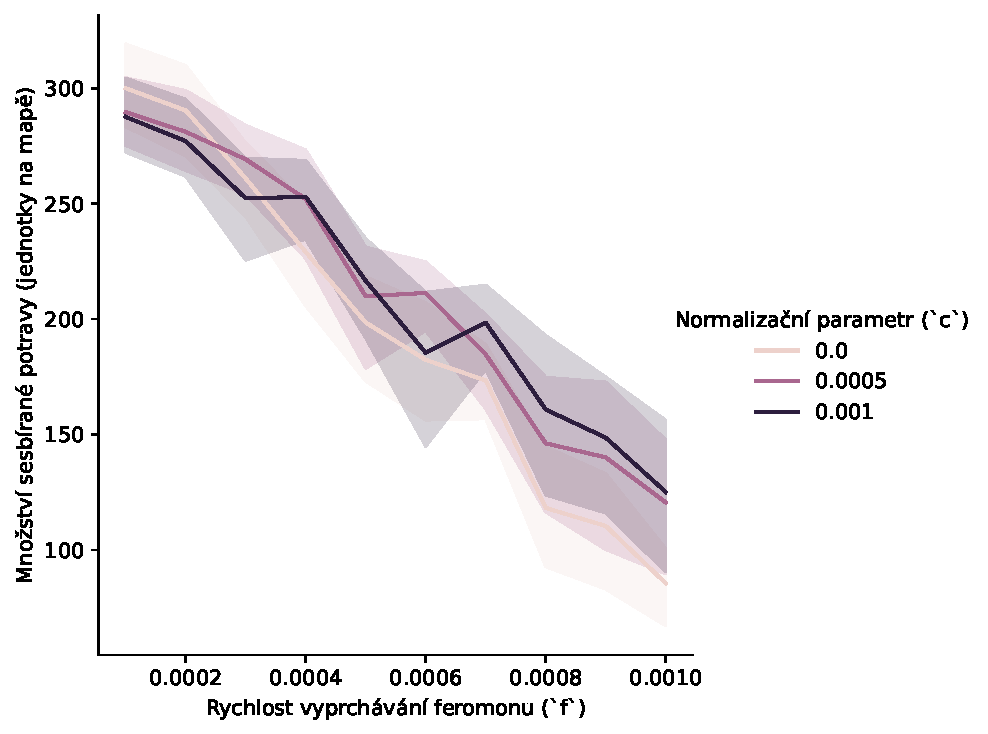
\includegraphics[width=0.9\linewidth]{images/grid_search_1_fade.pdf}
  \caption{\textbf{Množství sesbírané potravy v závislosti na parametrech `f` a `c`:}
  Množství sesbírané potravy je vyšší v případě částečně náhodného
  vlivu feromonu (varianty $c=0.0005$ a $c=0.001$). Množství sesbírané 
  potravy klesá téměř lineárně s rostoucí rychlostí vyprchávání feromonu 
  (parametr $f$).}
  \label{fig:grid_search_1_fade}
\end{figure}


\begin{figure}[tb]
  \centering
  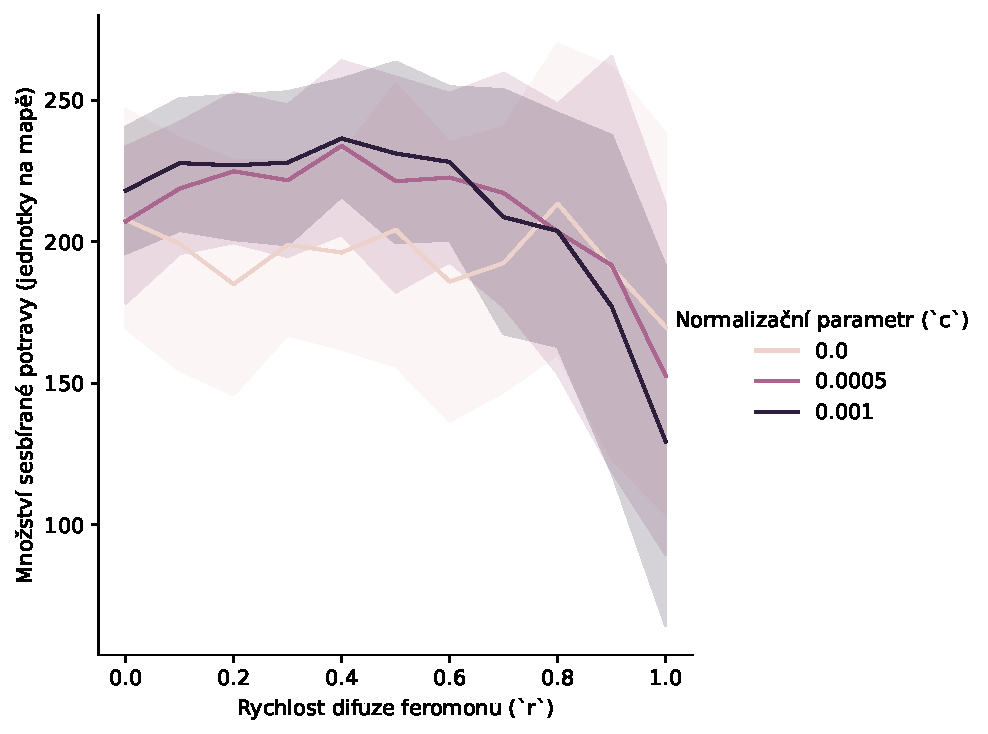
\includegraphics[width=0.9\linewidth]{images/grid_search_1_difusion.pdf}
  \caption{\textbf{Množství sesbírané potravy v závislosti na parametrech `r` a `c`:}
  Množství sesbírané potravy je vyšší v případě částečně náhodného
  vlivu feromonu (varianty $c=0.0005$ a $c=0.001$). Množství sesbírané 
  potravy není téměř ovlivněno změnou rychlosti difuze (parametr $r$). 
  Výrazný pokles pozorujeme až kolem hodnoty $0.8$ a vyšší.}
  \label{fig:grid_search_1_difusion}
\end{figure}


V druhé části výběru parametru jsme se zabývali pouze volbou parametru
rychlosti vyprchávání feromonu $f \in (0.0001, 0.001)$ 
se sousedními hodnotami rozdílnými o $0.0001$
a rychlosti difuze $r \in (0, 1)$ s hodnotami odlišujícími se o $0.1$. 
Porovnávali jsme množství sesbírané potravy za 
$8000$ iterací simulace. S pevně zvolenými parametry jako v případě 
první části a dále s parametrem $c = 0.0005$, jehož hodnotu jsme 
odvodili v první části. Z výsledků jsme podobně jako v případě 
první části vybrali 20 variant s nejvyšším počtem nasbírané potravy
a vypočítali aritmetický průměr hodnot parametrů $f$ a $r$. Vypočtené 
hodnoty jsou následující $f = 0.00021$ $r = 0.495$. Závislost vlivu 
parametrů je srovnatelný s výsledky první části a je znázorněn
grafy \ref{fig:grid_search_2_fade} a \ref{fig:grid_search_2_difusion}.


\begin{figure}[tb]
  \centering
  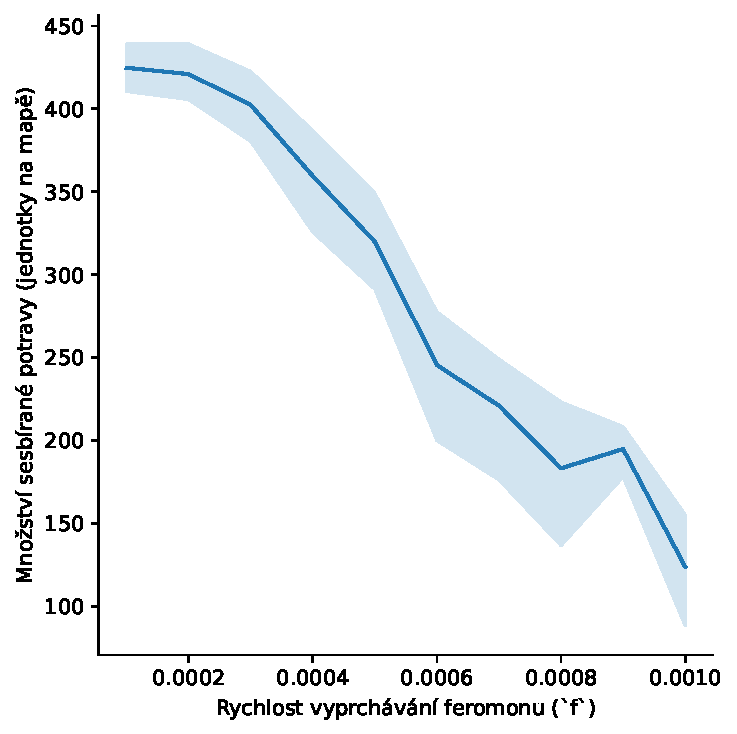
\includegraphics[width=0.9\linewidth]{images/grid_search_2_fade.pdf}
  \caption{\textbf{Množství sesbírané potravy v závislosti na rychlosti vyprchávání feromonu:}
  Množství sesbírané potravy klesá téměř lineárně s rostoucí 
  rychlostí vyprchávání feromonu (parametr $f$). Vyjímkou jsou hodnoty
  parametru $f$ do $0.0002$ u nichž je rozdíl téměř zanedbatelný.}
  \label{fig:grid_search_2_fade}
\end{figure}


\begin{figure}[tb]
  \centering
  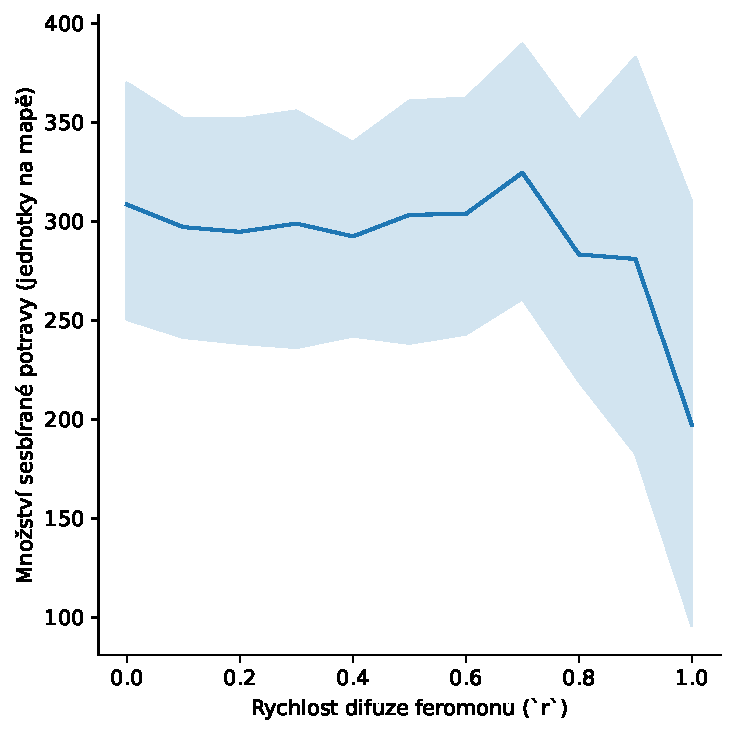
\includegraphics[width=0.9\linewidth]{images/grid_search_2_difusion.pdf}
  \caption{\textbf{Množství sesbírané potravy v závislosti na rychlosti difuze feromonu: }
  Množství sesbírané potravy není téměř ovlivněno změnou rychlosti 
  difuze (parametr $r$). Výrazný pokles pozorujeme až kolem hodnoty $0.8$ 
  a vyšší.}
  \label{fig:grid_search_2_difusion}
\end{figure}


\subsection{Popis experimentů}
\label{subsec:experiment_describtion} 
Hlavní část experimentů byla zaměřena na charakteristiku chování mravenců v
různých variantách prostředí s různým počtem jedinců (parametr $n$ v rozmezí 
$(20, 2000)$ se sousedními hodnotami lišícími se o $10$) a různou 
maximální vzdáleností pro detekci hledaného objektu 
(parametr $d$ v rozmezí $(0, 50)$ se sousedními hodnotami lišícími se o $1$). 
V experimentech jsme se zaměřovali na poměr sesbírané potravy vůči celkovému 
počtu potravy na mapě po uplynutí
$4000$ iterací simulace v rámci zkoumání charakteristiky chování mravenců
v různých prostředích a $8000$ iterací pro zkoumání vlastností pro různé hodnoty
parametrů pro $n$ a $d$. Na základě výběru parametrů 
(viz. část \ref{subsec:parameter_choice}) jsme 
pevně zvolili následující hodnoty zbylých parametrů:

\begin{itemize}
  \item $f = 0.00021$
  \item $p = 0.02$
  \item $r = 0.495$
  \item $c = 0.0005$
\end{itemize}


% Please use pisikabst.bst. You may your own *.bib file.
\clearpage
\bibliographystyle{pisikabst}
\bibliography{bibfile}

\section*{Doplňkové materiály}
Elektronická verze práce obsahuje doplňové materiály obsahující
animace simulací. Elektronická verze práce je dostupná na adrese
\url{https://github.com/dbeinhauer/ant_colony_model}


\end{document}